\documentclass[12pt,a4paper]{report}
\usepackage[utf8x]{inputenc}
\usepackage{graphicx}
\usepackage[labelfont=bf]{caption}
\usepackage{float}
\usepackage{hyperref}
\usepackage{amsmath}
\usepackage[export]{adjustbox}
\usepackage{color}
\usepackage{xcolor}

\usepackage{wrapfig}
\usepackage{lscape}
\usepackage{rotating}

\usepackage{tikz}
\usetikzlibrary{automata,positioning,arrows}

\usepackage{listings}
\lstset{basicstyle=\footnotesize, numbers=left, captionpos=b, frame=bt, linewidth=\textwidth, numberstyle=\tiny, showstringspaces=false}

\colorlet{punct}{red!60!black}
\definecolor{background}{HTML}{EEEEEE}
\definecolor{delim}{RGB}{20,105,176}
\colorlet{numb}{magenta!60!black}

\lstdefinelanguage{json}{
    basicstyle=\normalfont\ttfamily,
    numbers=left,
    numberstyle=\scriptsize,
    stepnumber=1,
    numbersep=8pt,
    showstringspaces=false,
    breaklines=true,
    frame=lines,
    backgroundcolor=\color{background},
    literate=
     *{0}{{{\color{numb}0}}}{1}
      {1}{{{\color{numb}1}}}{1}
      {2}{{{\color{numb}2}}}{1}
      {3}{{{\color{numb}3}}}{1}
      {4}{{{\color{numb}4}}}{1}
      {5}{{{\color{numb}5}}}{1}
      {6}{{{\color{numb}6}}}{1}
      {7}{{{\color{numb}7}}}{1}
      {8}{{{\color{numb}8}}}{1}
      {9}{{{\color{numb}9}}}{1}
      {:}{{{\color{punct}{:}}}}{1}
      {,}{{{\color{punct}{,}}}}{1}
      {\{}{{{\color{delim}{\{}}}}{1}
      {\}}{{{\color{delim}{\}}}}}{1}
      {[}{{{\color{delim}{[}}}}{1}
      {]}{{{\color{delim}{]}}}}{1},
}

% Windows
\graphicspath{{C:/Users/achantreau/Documents/GitHub/BEng-Individual-Project/Report/images/}}
\newcommand{\listings}{C:/Users/achantreau/Documents/GitHub/BEng-Individual-Project/Report/listings/}

% Linux
%\graphicspath{{/homes/ac6609/Documents/BEng-Individual-Project/Report/images/}}
%\newcommand{\listings}{/homes/ac6609/Documents/BEng-Individual-Project/Report/listings/}

\usepackage{fancyhdr}
\setlength{\headheight}{30pt}
\pagestyle{fancy}

\renewcommand{\chaptermark}[1]{\markboth{#1}{}}
\renewcommand{\sectionmark}[1]{\markright{#1}{}}

\fancyhf{}
\lhead{\fancyplain{}{\thepage}}
\chead{}
\rhead{\fancyplain{}{\textit{\leftmark}}}
\rfoot{\thepage}

\setlength\parindent{0pt}
\setcounter{page}{1}
\pagenumbering{roman}

\newcommand{\HRule}{\rule{\linewidth}{0.5mm}}
\newcommand{\me}{\mathrm{e}}

\begin{document}

%-----------------------------------------------------------
% TITLE SECTION
%-----------------------------------------------------------
\begin{titlepage}
\begin{center}

\textsc{\LARGE Imperial College London}\\[1.5cm]

\textsc{\Large BEng Individual Project - Final Report}\\[0.5cm]

% Title
\HRule \\[0.4cm]
{ \huge \bfseries jSCAPE - Java Self-assessment Center of Adaptive Programming Exercises \\[0.4cm] }

\HRule \\[1.5cm]

% Author and supervisor
\begin{minipage}{0.4\textwidth}
\begin{flushleft} \large
\emph{Author:}\\
Alexis \textsc{Chantreau}
\end{flushleft}
\end{minipage}
\begin{minipage}{0.4\textwidth}
\begin{flushright} \large
\emph{Supervisor:} \\
Dr.~Tristan \textsc{Allwood}
\end{flushright}
\end{minipage}

\vfill

% Bottom of the page
{\large \today}

\end{center}
\end{titlepage}

%-----------------------------------------------------------
% ABSTRACT SECTION
%-----------------------------------------------------------
\begin{abstract}
Programming is generally acknowledged to be a difficult discipline to learn, requiring problem solving skills, attention to detail and the ability to think abstractly. Yet, there is a definite interest in this subject as demonstrated by the number of students enrolling in computer science courses. \newline

In these courses, it is usually difficult for teachers and students to get an idea of how they are performing as they can only rely on a few assignments. This project aims to address this issue, by providing a solution which increases the amount of practise and feedback available to students and teachers.\newline

The result is a complete product in the form of jSCAPE (Java Self-assessment Center of Adaptive Programming Exercises) with core features consisting of providing programming exercises, displaying performance statistics, adapting the difficulty of exercises and generating exercises automatically.\newline

We used a difficulty category based algorithm, as well as concepts presented in Item Response Theory to adapt the difficulty of exercises to the student's ability.
\end{abstract}

%-----------------------------------------------------------
% ACKNOWLEDGEMENTS SECTION
%-----------------------------------------------------------
\renewcommand{\abstractname}{Acknowledgements}
\begin{abstract}
I would like to thank Dr. Tristan Allwood for proposing this project as well as providing guidance and support throughout. I would also like to thank my personal tutor, Prof. Duncan Gillies, for overseeing my time at Imperial. Last, but not least, I would like to thank my family, especially my parents for supporting me and always being there for me.
\end{abstract}

%-----------------------------------------------------------
% TABLE OF CONTENTS SECTION
%-----------------------------------------------------------
\tableofcontents

\newpage
\setcounter{page}{1}
\pagenumbering{arabic}

%-----------------------------------------------------------
% LIST OF FIGURES SECTION
%-----------------------------------------------------------
\listoffigures

%-----------------------------------------------------------
% LIST OF LISTINGS SECTION
%-----------------------------------------------------------
\renewcommand*{\lstlistlistingname}{List of Code Listings}
\lstlistoflistings

%-----------------------------------------------------------
% INTRODUCTION SECTION
%-----------------------------------------------------------
\chapter{Introduction}

\section{Motivation}
Programming is generally acknowledged to be a difficult discipline to learn, requiring problem solving skills, attention to detail and the ability to think abstractly. One could say that these skills are somewhat developed in high school during mathematics courses, but programming is still a ``beast" of its own. In addition, different programming paradigms exist, such as functional programming or imperative programming. Knowing how to program in Java can still make learning Haskell a difficult process.\newline

Yet, in this 21st century society, programming is definitely a useful skill to have, and there is an interest in the population to learn these skills. Indeed, this can be seen by the number of students enrolling in computer science courses at universities, or the increase in websites such as Codecademy\cite{Codecademy}, Coursera\cite{Coursera}, Udacity\cite{Udacity}, which provide online computer science/programming courses for free.\newline

In many of these situations, it is difficult for teachers, lecturers or course leaders to provide enough support through exercises, assignments and to monitor student's progress in such a way which allows them to modify their teaching to help struggling students. Indeed, teachers and students can generally only rely on a few homework assignments to get an idea of how they are doing. Coming up with a solution to increase the amount of practise and feedback would be beneficial to both students and teachers. \newline

Thus, there is a clear need to provide a platform for students to practise their programming skills and understanding of programming concepts, in a context of self-assessment only. In such a system, requiring teachers to come up with all the exercises by themselves can be both time consuming and ineffective: some exercises may not be challenging enough for certain top students, or on the contrary too difficult for struggling students, which can be discouraging for them.

\section{Objectives}
Having identified the problems associated with teaching and learning programming, we were led to formulating objectives in order to make the project successful and useful to the parties involved. \newline

The main objective of the project was to produce a web-based application to be used in self-assessing one's programming knowledge, whether it be in high school, at university or as part of an online course. For this application, four key features were identified:

\begin{itemize}
\item \textbf{Programming questions/exercises -} The web platform should allow students to practise their programming skills and understanding of programming concepts. There should be no limit to the number of questions a student can answer, so that if a student desires more practice, then he should be able to do that. Additionally, it should be possible for a specific set of people, such as teachers, lecturers or tutors, to add questions/exercises to the system.
\item \textbf{Progress tracking -} Designated people, such as teachers, lecturers or tutors, should have access to detailed statistics about the students performances. This will provide them with useful information about difficulties particular students, or the entire class, may be facing. In addition, the system should give feedback to the students, in the form of simple statistics, allowing them to identify their weak areas and thus improve on them.
\item \textbf{Adaptive difficulty -} The questions or exercises presented to the students should be suited to their ability. Not only will this stimulate the learning process, but it will also give a better indication of a student's understanding of the programming concepts being tested.
\item \textbf{Automated generation -} There should be a mechanism to allow for some degree of automated or semi-automated generation of exercises. This will provide a large supply of ``fresh" questions, so that students don't end up answering the same questions and memorizing the answers to them.
\end{itemize}

While investigating existing solutions (chapter \ref{chap:related-work}) we found out that some of these features were less common than others. The availability of programming exercises and progress tracking are very essential in such systems, therefore many of the related software we looked at implemented these features. On the other hand, relatively few tools integrated some form of adaptive difficulty. Finally, almost none of the tools featured automated generation of questions, opting instead to allow exercises to be added manually to the system, or downloaded from existing exercise banks.

\section{Contributions}
Within the context given above, this project makes the following contributions:
\begin{itemize}
\item \textbf{jSCAPE}: a web application for students, named Java Self-assessment Center of Adaptive Programming Exercises, with the following features:
      \begin{itemize}
      \item[-] the ability to view programming exercises and answer them while receiving feedback, a so called form of self-assessment.
      \item[-] graphs, tables and pie charts displaying statistical data on the student's performance.
      \item[-] three different exercise selection algorithms, that decide which is the best exercise to present to the student.
      \end{itemize}
\item \textbf{Admin tool}: a tool for teachers/lecturers/tutors for:
      \begin{itemize}
      \item[-] displaying student performance statistics.
      \item[-] displaying exercise statistics.
      \item[-] defining exercise categories.
      \item[-] adding exercises manually.
      \item[-] generating exercises automatically.
      \end{itemize}
\end{itemize}

\section{Report Structure}
Chapter \ref{chap:background} will present the theoretical basis for this project and the concepts necessary to follow the implementation details of the system.\newline

Chapter \ref{chap:related-work} will give an overview of related work, and will mention how these influenced the design of jSCAPE, in particular which features would be useful for such as system.\newline

Chapter \ref{chap:jscape-system} will present the jSCAPE system in detail, showing all the features which are available.\newline

Chapter \ref{chap:implementation} will cover the design and implementation details of the jSCAPE system, in particular how the difficulty of exercises is adapted to the student's ability and how exercises can be automatically generated.\newline

Chapter \ref{chap:evaluation} will contain the results of evaluating jSCAPE as a whole, and its different components. \newline

Chapter \ref{chap:conclusion} summarises the achievements of the project and discusses possible extensions that can be made to the system in the future.


%-----------------------------------------------------------
% BACKGROUND SECTION
%-----------------------------------------------------------
\chapter{Background}
% Add maximum likelihood background explanation
% Add Bayesian probability background explanation
%Add note to say that we use the word examinee to mean someone taking a test although the test may not be an exam per say.

\section{Computer Based Tests}
CBT abbreviation
- offers advantages such as being able to display higher quality visuals such as pictures, videos, graphs, etc...
- low paperwork, everything is stored on the computer
- automatic grading, less work for teachers
- generation of statistics is made easier by the fact that the data can be processed by the computer
- nowadays a lot of learning is done on computer systems, and children are used to dealing with computers so assessment through this medium is advantageous. \newline

CBTs are typically "fixed-item" tests where all the students answer the same set of questions,  usually provided by the person responsible for the assessment. This isn't ideal since students can be presented with questions that are too easy or too difficult for them to answer. Consequently, the results of the test won't give a very accurate representation of a student's ability, and for this reason, these types of tests aren't extremely useful. This problem lead to research and the development of computerized adaptive testing (CAT).

\section{Computerized Adaptive Testing}
\label{sec:CAT}
Computerized adaptive testing (CAT), also called \textit{tailored testing}, is a form of computer-based testing which administers questions (referred to as \textit{items} in the psychometrics literature) of the appropriate difficulty by adapting to the examinee's ability.
For example, if an examinee answers an item correctly, then the next item presented will higher on the difficulty scale. On the other hand, if they answer incorrectly, they will be presented with an item lower on the difficulty scale. \newline

From an architectural perspective, a computerized adaptive test (CAT) consists of five components \cite{CAT-Framework}:

\subsubsection{1. Calibrated item pool}
An item pool is needed to store all the items available for inclusion in a test. This item pool must be calibrated with a psychometric model. During this phase, the item parameters are estimated according to the chosen model and scaled to fit with already existing items. Usually, the psychometric model employed in these systems is called Item Response Theory (IRT) (section \ref{subsec:IRT}). Calibration is a complex process, and to be done accurately it requires a considerable amount of data. Typically, it is performed by psychometricians, aided by expensive and sophisticated calibration software.

\subsubsection{2. Starting point}
Initially, when zero items have been administered, no information is known about the examinees and so the CAT is unable to estimate their ability. As a result, the item selection algorithm will fail to choose the next item to be administered.
If there is previous information available, for example an examinee's ability estimate in a closely related subject, then this can be input into the system to form the starting point configuration. Often this data isn't available or too costly to collect, so the CAT's initial ability estimate for the examinee corresponds to the mean on the ability scale - hence the first item presented will be of average difficulty.

\subsubsection{3. Item selection algorithm}
The item selection algorithm chooses the next item to present to the examinee based on the ability estimate of the examinee up to that point. Several methods exist and largely depend on the psychometric model in use. One of the most commonly used methods is the \textit{maximum information method} (section \ref{subsec:IRT}), which selects the item which maximizes the information function with respect to the estimated ability at that point.

\subsubsection{4. Scoring algorithm}
The scoring algorithm refers to the steps taken to update the examinee's ability estimate after an item has been answered. The two most commonly used methods are \textit{maximum likelihood estimation} (section \ref{subsec:IRT}) and \textit{Bayesian estimation} (section \ref{subsec:IRT}).

\subsubsection{5. Termination criterion}
The termination criterion specifies when the CAT should finish. For example the CAT can terminate when the change in the ability estimate after each iteration is below a certain threshold, or when time has run out, or when $N$ items have been administered, etc... Obviously, the CAT shouldn't be terminated too early, so as to allow enough time to estimate the examinee's ability with acceptable accuracy.

\begin{figure}[H]
\centering
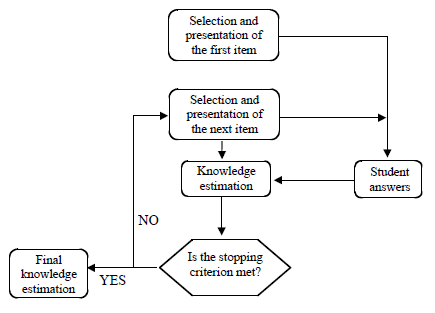
\includegraphics[scale=1]{cat_flowchart}
\caption{Flowchart of an adaptive test. Adapted from \cite{SIETTE}.}
\label{fig:cat_flowchart}
\end{figure}

The flowchart in figure~\ref{fig:cat_flowchart} corresponds to components 2-5, and illustrates the basics of the algorithm implemented in CAT. \cite{CAT-Wiki} gives a more detailed description of the procedure:
\begin{itemize}
\item[1.] The pool of items that haven't been administered yet is searched to determine the best item to present to the examinee, according to the current estimation of his ability.
\item[2.] The chosen item is presented to the examinee, who then answers it correctly or incorrectly.
\item[3.] The ability estimate is updated, based upon this new piece of information and the previous ability estimate.
\item[4.] Steps 1–3 are repeated until a termination criterion is met.
\item[5.] The algorithm returns a final ability estimate for the examinee's performance along with a confidence level: a percentage value indicating how accurate the estimate is.
\end{itemize}

CATs offer several advantages over traditional CBTs. As a result CATs have been used in many areas\cite{CAT-Areas}, such as education, job hiring, counselling, clinical studies, etc... Since CATs administer items by adapting to the examinee's ability, the test-taking experience ends up being a more positive one. Indeed, examinees won't have to deal with answering items which are too difficult or too easy compared to their ability level, a problem which appears in traditional CBTs.\newline

In addition, by administering only those items which will yield additional information, CATs end up being more accurate in estimating an examinee's ability level. This contrasts with CBTs which usually provide the best precision for examinees of medium ability, whereas extreme scores end up being less accurate.\newline

Lastly, CATs can come up with an ability estimate much quicker and with fewer administered items when compared to traditional CBTs. Indeed, an adaptive test can typically be shortened by 50\% and still maintain a higher level of precision than a fixed version.\cite{Weiss1984}
\newline

Despite the advantages mentioned above, CATs have some limitations. A frequent complaint is that an examinee isn't allowed to go back and change his answer to a past item. This limitation exists to prevent the examinee from intentionally answering items incorrectly to make subsequent items easier, and then going back and selecting the correct answers to achieve a perfect score. For similar reasons, it isn't possible to skip items, the examinee must select an answer to move on to the next item.\newline

The second issue has to do with the items themselves. First of all, there is the need for a large bank of items to cater to all ability levels. Developing an item pool of sufficient size can be very time consuming. David J. Weiss writes in \cite{Weiss1985} that item pools with 150-200 items are to be preferred, although 100 high quality items can sometimes be enough to achieve adequate estimations of ability levels.

Secondly, for the CAT to be of good quality the item pool needs to be calibrated accurately. This requires pre-administering the items to a sizeable sample and then simultaneously estimating all the item parameters for each item. The guidelines in \cite{CAT-Primer} suggest that sample sizes may be as large as $1000$ examinees. This phase is costly, time consuming and often times simply unfeasible.\newline

Lastly, item exposure is a possible security concern. Sometimes particular items may be presented too often and become overused. This may result in examinees becoming familiar with them and sharing them to other examinees of the same ability level, thus corrupting the results of the test. This problem can be solved to some extent by modifying the item selection algorithm to include some exposure control mechanism.\newline

A brief overview of CATs was given in this section. All of these concepts will be explored in more detail in item response theory (section \ref{subsec:IRT}) and in the implementation of adaptive testing in jSCAPE (chapter XX?).

\section{Probabilistic Test Theory}
In this section we go over a few topics in probability and how they can be implemented successfully in the area of computer assessments.

\subsection{Likelihood and Maximum Likelihood Estimation}
Although the terms probability and likelihood are used interchangeably in every day life, in statistics a distinction can be made.\newline

For any stochastic process, let us denote the observed outcomes as $x$ and the set of parameters as $\theta$. When we say probability, we want to calculate $P(x | \theta)$, i.e. the probability of observing the outcomes $x$ given specific values for the set of parameters $\theta$. \newline



In more mathematical terms, we have:
$$L(\theta | x) = P(x | \theta)$$

To highlight the distinction we illustrate with an example of how the two terms are used. If we consider a dice, a possible parameter is the fairness of the dice, while possible outcomes are which values are displayed after a roll. For instance, if a fair dice is rolled 5 times, what is the \textit{probability} that a 6 will show up on every roll? If a dice is rolled 5 times and lands on 6 every roll, what is the \textit{likelihood} that the dice is fair? \newline

Maximum likelihood estimation refers to a method of statistical inference where one can find the set of parameter values ($\theta$) which are most \textit{likely} given the observed outcomes ($x$). As mentioned in the name of the method, this is done by finding the parameter values which maximize the likelihood function $L(\theta | x)$.

\subsection{Bayes probability theory}
% Add maximum likelihood background explanation
% Conditional probability quick overview?
% Add Bayesian probability background explanation
% Bayesian networks
% Latent variables ?

\subsection{Item Response Theory}
\label{subsec:IRT}
We mentioned in section \ref{sec:CAT} that Item Response Theory (IRT) is usually the psychometric model of choice when developing a CAT, e.g. the Graduate Record Examination (GRE) and Graduate Management Admission Test (GMAT). CATs can still be implemented with Classical Test Theory but they offer less sophistication and less information to evaluate/improve the reliability of the test, making IRT the superior choice. \newline

IRT attempts to model the answer to an item as a mathematical model. \newline

Several IRT models have been developed over the years to address the different types of tests that exist, e.g. multiple choice exams, agreement questionnaires (Likert scale), etc... These models all seek to achieve the same goal, modelling the examinee's ability on some ability scale, but they differ in the number of parameters associated with each item. We now take a greater look at these different models:

\subsubsection{The one-parameter logistic model}
\begin{equation} \label{eq:1PL-IRF}
P(\theta) = \frac{1}{1 + \me^{-(\theta - b)}}
\end{equation}

Equation \eqref{eq:1PL-IRF} shows the item response function for the one-parameter logistic model (1PL). 

\subsubsection{The two-parameter logistic model}
\begin{equation} \label{eq:2PL-IRF}
P(\theta) = \frac{1}{1 + \me^{-1.7a(\theta - b)}}
\end{equation}

Equation \eqref{eq:2PL-IRF} shows the item response function for the two-parameter logistic model (2PL). 

\subsubsection{The three-parameter logistic model}
\begin{equation} \label{eq:3PL-IRF}
P(\theta) = c + \frac{1 - c}{1 + \me^{-1.7a(\theta - b)}}
\end{equation}

Equation \eqref{eq:3PL-IRF} shows the item response function for the three-parameter logistic model (3PL). 

\subsubsection{Estimating the ability}
In section \ref{sec:CAT}, when discussing scoring algorithms, we saw that the two most common methods for ability estimation were \textit{maximum likelihood estimation} and \textit{Bayesian estimation}.\newline

In the \textit{maximum likelihood estimation} method, we need to define a likelihood function in terms of the ability level ($\theta$) we are trying to estimate:

\begin{equation} \label{eq:Trait-estimation}
L(\theta | \textbf{u}) = L(\theta | u_1, ..., u_n) = P(u_1, ..., u_n | \theta) = \prod_{i=1}^n P_i(\theta)^{u_i}(1 - P_i(\theta))^{(1 - u_i)} ,
\end{equation}

where $\textbf{u}=(u_1, ..., u_n)$ is called the reponse vector for an examinee, that is $u_i=1$ if the examinee answers the i$^\text{th}$ item correctly, and $u_i=0$ if the examinee answers the i$^\text{th}$ item incorrectly. $P_i(\theta)$ corresponds to the probability of answering the i$^\text{th}$ item correctly when the ability level is $\theta$, and thus $1 - P_i(\theta)$ gives the probability of answering the i$^\text{th}$ item incorrectly when the ability level is $\theta$. \newline

Now that the likelihood function is defined, we can apply maximum likelihood estimation to find the ability level which is most likely given the examinee's response vector. Let us illustrate with a very simplistic example where ability levels are discrete values between $-1$ and $+1$. We would iterate through these ability levels and compute the following values, for example:
\begin{align*}
L(\theta=-1 | \textbf{u}) &= 0.001 \\
L(\theta=+0 | \textbf{u}) &= 0.012 \\
L(\theta=+1 | \textbf{u}) &= 0.054
\end{align*}

The likelihood function is maximized when $\theta = +1$, and so this is the maximum likelihood estimate for $\theta$. In a CAT, and based on the examinee's response vector \textbf{u}, the system would assign $+1$ as the ability level for that examinee.\newline

The \textit{Bayesian estimation} method is also somewhat based on the likelihood function and therefore very similar to \textit{maximum likelihood estimation}.........


\subsubsection{Item information}

\section{Summary}
We have gone over types of computer based assessment and how they differ from regular assessment techniques. We have also provided an overview of the theoretical components and probability concepts which will be implemented in jSCAPE (chapter xx?).


%-----------------------------------------------------------
% RELATED WORK SECTION
%-----------------------------------------------------------
\chapter{Related Work}
\label{chap:related-work}
With the rise of computer usage in today's society, they have quite naturally made their way over to education. As such, web-based, computer-based and adaptive assessment systems have been investigated and researched quite thoroughly over the years. The result of this research is numerous tools and software which provide students the opportunity to practise their programming skills, whether it be by writing code or answering programming questions, in an environment which tracks their progress. Almost all of these tools provide the basic features, that is the programming exercises themselves, and a component to view statistics or student results. Some of them distinguish themselves by adding useful and not so common features such as adaptive difficulty. From all the solutions we looked at, very few provided automate exercise generation, and for those who did, their approach was only limited to extremely simple exercises. \newline

We have looked at quite a few solutions such as ELP (Environment for Learning to Program) and CourseMaster, which have the very basic features. We do not go into detail about how these solutions operate since the details are quite straightfowrad and not very interesting. Instead we focus on software which has approached the adaptive difficulty problem, and look into how they did so.\newline

In this section we look at the related software which has influenced the design and implementation of our proposed solution, jSCAPE.

\section{Programming Adaptive Testing}
\label{sec:PAT}
PAT\cite{PAT} is a web-based adaptive testing system, developed in ActionScript/Flash, for assessing students' programming knowledge in Greek high schools. \newline

The assessment is carried out by presenting students with 30 questions from various chapters of the introductory programming course. Some of the questions supported by the PAT system are true/false questions, multiple choice questions, gap filling in a piece of code, questions involving diagrams and questions where one has to determine the behaviour of a piece of code.\newline

In PAT, questions are classified into different difficulty categories. Category A is for easy questions, category B is for intermediate questions and category C is for difficult questions. PAT seeks to adapt the difficulty of the questions to the student's ability, by choosing questions of the appropriate difficulty category.

\begin{figure}[H]
\centering
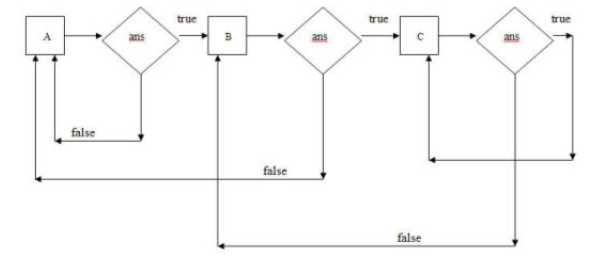
\includegraphics[width=\textwidth,height=\textheight,keepaspectratio]{PAT_adaptive_sequence}
\caption{Adaptive sequence of questions in PAT. (Source:\cite{PAT})}
\label{fig:PAT_adaptive_sequence}
\end{figure}

Figure \ref{fig:PAT_adaptive_sequence} shows the possible adaptive sequences. This algorithm is quite simplistic, every correct answer leads to a promotion to the next level of difficulty until no further promotions are possible. Likewise, every incorrect answer leads to a demotion to a lower level of difficulty until no further demotions are possible.\newline

At the end of the test, the system shows the student's total number of correct answers out of 30 and how well the student performed on each chapter. Also, PAT classifies the student into one of three programming skill levels based on their final score and a weighted score, where the difficulty of the questions answered correctly is considered. These results are available to both students and teachers so that they can be used to improve performance later on in the school year.\newline

We feel that the adaptive algorithm increases the difficulty of questions too quickly and doesn't take into account guessing or possible slip ups from students. This limitation can be circumvented by, for instance, requiring a number of correct answers at the current difficulty level before progressing to the next one.\newline

PAT only provides assessment at specific times throughout the school year and no opportunity for students to practice and self-assess in their own time. In addition, it isn't possible for teachers to upload their own questions to the system. The question bank remains static and contains 443 questions. Lastly, the authors of PAT admit that the statistical data available to students and teachers is fairly limited, and that improvements should be pursued in future work.

\section{SIETTE}
\label{sec:SIETTE}
SIETTE\cite{SIETTE-small} (System of Intelligent Evaluation Using Tests for Tele-education) is a web based environment for generating and constructing adaptive tests. It has been used with great success in courses from the computer science engineering school, the telecommunication engineering school and the philosophy faculty, all at the University of Malaga, Spain.\newline

SIETTE is a vast system, and at the time of publication (2005) it contained information about $15000$ student test sessions, and the knowledge base contained 84 subjects, 1852 topics, 3820 question and 220 tests.\newline

SIETTE is designed to be used by both students and teachers. Teachers use the system to create tests, define the subject topics, the questions and their parameters. Students use the system to take the tests specified by the teachers. The tests can be used for self-assessment, where the correction is shown immediately after the student has answered. Hints and more extensive feedback are also available in this mode. Or, the tests can be used as exams, where the score counts towards the student's final grade. In this mode, hints and feedback aren't provided. It is important to note that tests have a fixed number of questions, thus, new tests must be created every time a student runs out of practice.\newline

As mentioned earlier, SIETTE constructs adaptive tests, therefore, when a student answers a question, his ability is re-estimated and the next question is selected accordingly. Implementation of this is done by using item response theory in the computerized adaptive testing framework.\newline

SIETTE uses the three-parameter logistic (3PL) model and measures the student's knowledge in terms of a discrete random variable $\theta$, which ranges from 0 to $K-1$, where $K$ is the number of discrete knowledge levels. When it comes to creating items, the guessing parameter $c$ is determined automatically, whereas the other two parameters must be entered by the teacher. The discrimination parameter ($a$) must be a number between $0.5$ and $1.5$. The difficulty parameter must be a natural number between 0 and $K-1$. A few years after the SIETTE paper was published, the authors added an item calibration tool because teacher estimates of item parameters are never very accurate.\newline

To estimate students' knowledge level, SIETTE uses the Bayesian estimation method (section \ref{subsec:IRT}) with a knowledge distribution per student, per topic. Also, SIETTE provides teachers with the option of choosing different item selection procedures for tests, such as random selection, difficulty-based selection and bayesian selection.

\begin{figure}[H]
\centering
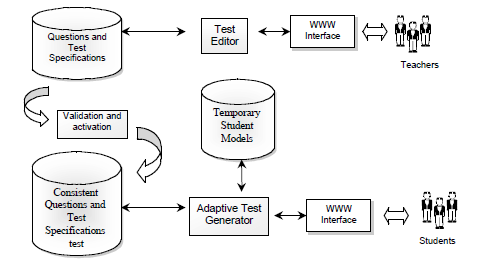
\includegraphics[width=\textwidth,height=\textheight,keepaspectratio]{siette-architecture}
\caption{SIETTE Architecture. (Source:\cite{SIETTE})}
\label{fig:siette-architecture}
\end{figure}

Figure \ref{fig:siette-architecture} gives on overview of the SIETTE architecture. The system is comprised of several components\cite{SIETTE-components}:
\begin{itemize}
\item The \textit{knowledge base}: where tests, topics and questions are stored. Some supported question types are true/false, multiple choice, multiple response and fill-in-the-gap. More interactive questions also exist, implemented as Java applets, where one has to color parts of a map, or move around objects so that they appear chronologically, for example.
\item The \textit{student model repository}: a collection of student models, where information about students' knowledge level estimation, which questions they answered, etc... is stored.
\item The \textit{student workspace}: a web interface where students take tests.
\item The \textit{test editor}: a tool where teachers can define tests, topics, questions.
\item The \textit{result analyzer}: a tool which presents graphical data about students' performance, knowledge estimation levels, etc...
\item The \textit{item calibration tool}: a module used to calibrate items by determining the item parameters (difficulty, discrimination and pseudo-chance).
\end{itemize}

SIETTE is a large and complex system, containing many useful features relevant to the area of web-education, and going through all of these wouldn't be possible. Since SIETTE has been used to such success in university courses we decide to inspire ourselves from this system, especially for the implementation of the adaptive difficulty component. Details about the algorithms used in SIETTE, and hence jSCAPE, can be found in section \ref{sec:implementing-cat}, with Java code to illustrate. However, SIETTE does not provide mechanisms to automatically generate exercises, and so we shall define our own algorithms for this.

\section{Summary}
We have looked at some of the relevant work in the field of computer based education and assessment. We saw that PAT provided a simple algorithm for increasing or decreasing the difficulty of exercises, and so an improved version of this algorithm will feature in jSCAPE. We also saw that SIETTE provided many of the features we set out to replicate in jSCAPE, therefore particular parts of our implementation will be inspired by SIETTE.\newline

SIETTE is the most complete system we have come across while doing research for this project. Moreover, examining some existing solutions which haven't been detailed in this section, has given us insight into the most common features available in these types of systems. \newline

In the next chapter we present the system developed as part of this project: jSCAPE. 

%-----------------------------------------------------------
% JSCAPE SYSTEM SECTION
%-----------------------------------------------------------
\chapter{The jSCAPE System}

The jSCAPE system is designed for two groups of intended users: students and teachers/lecturers. 

\begin{figure}[H]
\centering
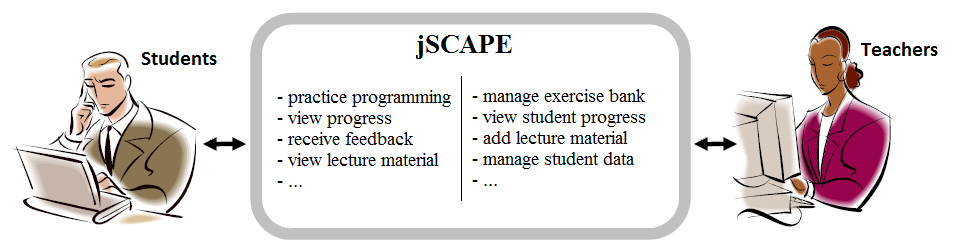
\includegraphics[scale=0.60]{jscape_use_case}
\caption{Use case diagram of the jSCAPE system.}
\label{fig:jscape_use_case}
\end{figure}


\section{Student view}
As illustrated in figure \ref{fig:jscape_use_case}, students can practice their understanding of programming concepts through answering exercises... We now show the complete features of the system.

\subsection{Practicing programming}

\subsection{Tracking your progress}

\section{Teacher view}
The teacher's main access to the system is through the jSCAPE admin tool. 

\subsection{Tracking student progress}

\subsection{Managing the exercise bank}



%-----------------------------------------------------------
% IMPLEMENTATION SECTION
%-----------------------------------------------------------
\chapter{Design and Implementation}
\label{chap:implementation}
Figure \ref{fig:three-tier-architecture} gives an overview of the three-tier architecture of the jSCAPE system, the relationships between each of the main components, and some of the tasks that they perform. The student view is implemented as a JavaFX applet embedded into the web browser. It communicates with a custom written Java application server using a custom built communication protocol. Finally, the application server also connects to a PostgreSQL database, to perform the standard read and write operations. \newline

\begin{figure}[H]
\centering
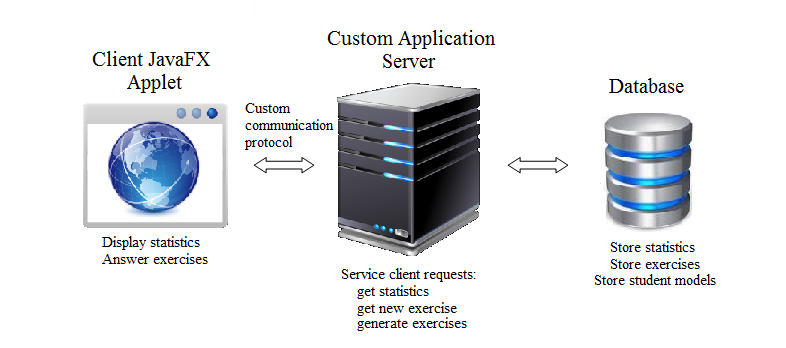
\includegraphics[width=\textwidth,height=\textheight,keepaspectratio]{three-tier-architecture}
\caption{Three tier architecture of the jSCAPE system.}
\label{fig:three-tier-architecture}
\end{figure}

The jSCAPE admin tool isn't really part of the core system's three tier architecture. The component was written later on to facilitate certain functions such as analyzing results and exercise bank management. To do so, it connects directly to the database to read or write information. The admin tool is shown in figure  \ref{fig:admin_tool_architecture}, along with its sub-components: the Results Analyzer, for displaying statistics in graphical form, and the Exercise Generator, for generating new exercises.

\begin{figure}[H]
\centering
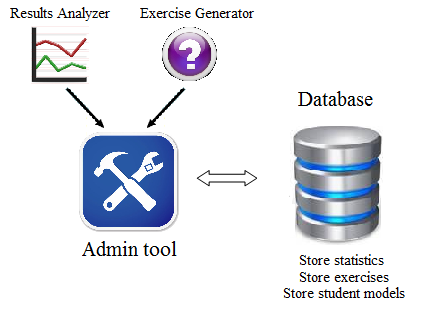
\includegraphics[scale=0.8]{admin_tool_architecture}
\caption{Architecture of the jSCAPE admin tool}
\label{fig:admin_tool_architecture}
\end{figure}

In the rest of this chapter we justify our design choices and discuss the implementation of the various components and features of the jSCAPE system.

\section{Technology choices}
Most software in the area of computer based education is web-based, as demonstrated by the review of related work in chapter \ref{chap:related-work}. We decided to follow this trend, as it makes deployment easier, and because students are usually quite familiar with web browsers. Therefore, the three-tier architecture of web client, server and database was the natural model of choice for creating such a system. There are multiple technologies which can be used to develop the client side. Some of these are HTML5, CSS, Javascript, Flash, and Java applets.\newline

We decided to take the approach of Java applets because we have had a lot of experience with developing large scale programs in this language. In addition, in our opinion, Java applets are better for creating rich web applications which resemble desktop applications. Websites require the user to continuously click links, and load web pages to access a feature, and we think that this model isn't suitable for developing jSCAPE. Finally, implementing jSCAPE as an applet allows it to run in Java web start mode or as a stand alone desktop application, thanks to the Java deployment framework. \newline

However, regular Java applets use the Swing library for GUIs, and as a result, the interface doesn't end up being user-friendly or visually appealing. This is certainly a problem, because although the application can present powerful and useful features, students will only use it if the interface is intuitive and aesthetically pleasing\cite{Interface-study}. \newline

This realisation led us to researching libraries which could improve the interfaces of Java applets, and discovering JavaFX. JavaFX is intended as a replacement for the Swing GUI library, and is designed to provide a lightweight, hardware-accelerated Java UI platform for creating rich internet applications\cite{JavaFX}. The JavaFX library includes a powerful and visually appealing statistics package, with support for pie charts, bar charts, line charts, scatter charts, tables, etc... which was more than enough to implement the statistics tracking and displaying component of jSCAPE. In addition, this would allow us to easily add more displayable statistics in the future (section \ref{sec:future-work}), if required. \newline

JavaFX also provides the functionality of embedding a \textsf{WebView}, a browser component which supports HTML5, CSS and Javascript, into the applet. We found that this could be an interesting feature to use for developing exercises with variety and interactivity, For instance, this component is used in the Binary Tree exercises to display the binary trees (section 5.??). \newline

Every web application needs some sort of server to handle web client requests. We looked at Java Server Pages (JSP) and Java Servlets, but the setup and organization required to make them work seemed to be too much work for the very little advantages they offered. Instead we opted to write our own Java server because this would offer more control for handling requests and more flexibility for extensions in the future. In addition, the time and amount of code required to write a functional server was very minimal. Indeed, the basic components of our custom built server fit into approximately 300 lines of code. \newline

A database is needed for permanent storage of the system's state, student models, exercises, etc... Thus, to do this, we use a PostgreSQL database and connect to it using the associated Java Database Connectivity (JDBC) driver. \newline

Throughout this chapter, we will give more detail about which tables are maintained by the system, and how they are used. In addition, we will introduce some other technologies and libraries used in this project later on, when we look at the exercise generation and display processes.
\section{Design}
This section describes the design of the jSCAPE system.

\subsection{Client}
\begin{figure}[H]
\centering
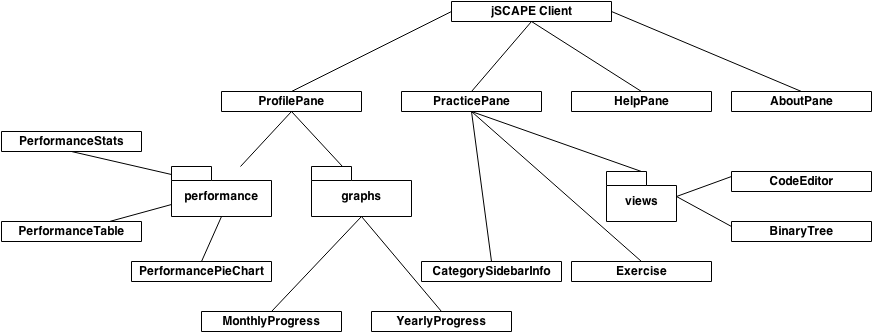
\includegraphics[width=\textwidth,height=\textheight,keepaspectratio]{class_diagram_client}
\caption{Class diagram of the jSCAPE client.}
\label{fig:class_diagram_client}
\end{figure}

Figure \ref{fig:class_diagram_client} shows the class diagram of the jSCAPE client, which is what is embedded into the web browser, and displayed to students. We briefly describe the classes:
\begin{itemize}
\item \textsf{ProfilePane}: The Profile tab of the application.
      \begin{itemize}
      \item[-] \textsf{performance} package:
               \begin{itemize}
               \item[-] \textsf{PerformanceStats}: Stores performance statistics, i.e. exercise category, correct answers, wrong answers.
               \item[-] \textsf{PerformanceTable}: Table wrapper to display \textsf{PerformanceStats} objects.
               \item[-] \textsf{PerformancePieChart}: PieChart wrapper to display \textsf{PerformanceStats} objects.
               \end{itemize}
      \item[-] \textsf{graphs} package:
               \begin{itemize}
               \item[-] \textsf{MonthlyProgress}: StackedBarChart wrapper to display monthly progress statistics.
               \item[-] \textsf{YearlyProgress}: StackedBarChart wrapper to display yearly progress statistics.
               \end{itemize}
      \end{itemize}
\item \textsf{PracticePane}: The Practice tab of the application.
       \begin{itemize}
       \item[-] \textsf{Exercise}: Stores an exercise and information such as exercise ID, description, choices, solution, display values.
       \item[-] \textsf{CategorySidebarInfo}: Stores information to create the sidebar of an exercise window.
       \item[-] \textsf{views} package contains the classes to render exercises in the left part of the Practice tab:
                \begin{itemize}
                \item[-] \textsf{BinaryTree}: Component capable of drawing binary trees.
                \item[-] \textsf{CodeEditor}: Component capable of displaying programming code in a code editor.
                \end{itemize}
       \end{itemize}

\item \textsf{HelpPane}: The Help tab of the application, displays the manual.

\item \textsf{AboutPane}: The About tab of the application, displays information about what the application does.
\end{itemize}

The jSCAPE client accounts for approximately 2500 lines of code.

\subsection{Server}
\begin{figure}[H]
\centering
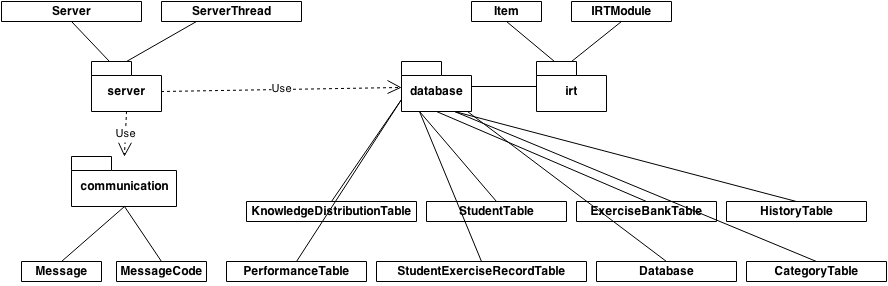
\includegraphics[width=\textwidth,height=\textheight,keepaspectratio]{class_diagram_server}
\caption{Class diagram of the jSCAPE server.}
\label{fig:class_diagram_server}
\end{figure}

Figure \ref{fig:class_diagram_server} shows the class diagram of the jSCAPE server, and the database classes the server uses to satisfy client requests. We briefly describe the classes:
\begin{itemize}
\item \textsf{server} package:
      \begin{itemize}
      \item[-] \textsf{Server}: The server, creates \textsf{ServerThread}s to handle client connections.
      \item[-] \textsf{ServerThread}: Receives requests from the client(s), performs work and replies to the client(s).
      \end{itemize}
\item \textsf{communication} package:
      \begin{itemize}
      \item[-] \textsf{Message}: A data structure to hold information. This is the unit which ``travels" between the client and server, and vice-versa.
      \item[-] \textsf{MessageCode}: Enum to identify structure and format of a \textsf{Message}.
      \end{itemize}     
\item \textsf{database} package:
      \begin{itemize}
      \item[-] \textsf{Database}: Manages the connection info and hands out connections to the components that wish to access the physical database.
      \item[-] \textsf{StudentTable}: Stores profile information of students, login names, passwords, etc...
      \item[-] \textsf{CategoryTable}: Stores the exercise categories, their description and associated lecture notes or helpful website links.
      \item[-] \textsf{PerformanceTable}: Stores performance statistics, such as correct answers and wrong answers, of students for the different exercise categories.
      \item[-] \textsf{HistoryTable}: Stores performance statistics of students for each day they used the system.
      \item[-] \textsf{ExerciseBankTable}: Stores the exercises, some exercise metrics and difficulty parameters.
      \item[-] \textsf{StudentExerciseRecordTable}: Stores which exercises students have answered and whether they got it correct or incorrect.
      \item[-] \textsf{KnowledgeDistributionTable}: Stores the knowledge distribution of the student per exercise category, in the case that Item Response Theory is used.
      \end{itemize}
\item \textsf{irt} package: This package is a Java implementation of Item Response Theory.
      \begin{itemize}
      \item[-] \textsf{Item}: An IRT item, which stores an exercise ID and item parameters.
      \item[-] \textsf{IRTModule}: Implements IRT concepts such as the item response function, the item information function, ability estimation, etc...
      \end{itemize}
\end{itemize}

\subsection{Exercises and exercise generators}
\begin{figure}[H]
\centering
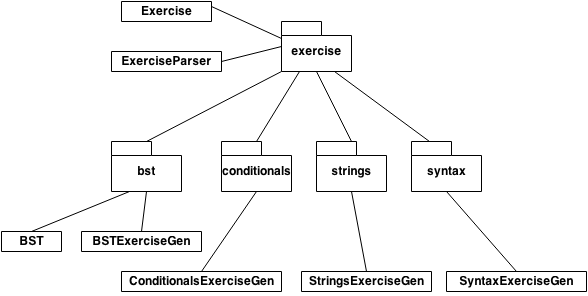
\includegraphics[width=\textwidth,height=\textheight,keepaspectratio]{class_diagram_exercises}
\caption{Class diagram of the currently implemented exercise generators.}
\label{fig:class_diagram_exercises}
\end{figure}

Figure \ref{fig:class_diagram_exercises} shows the class diagram for exercises and the implemented exercise generators, at the time of writing this report. We briefly describe the classes:
\begin{itemize}
\item \textsf{Exercise}: Stores an exercise and information such as exercise ID, description, choices, solution, display values.
\item \textsf{ExerciseParser}: Special XML parser to decode the exercise format and return an \textsf{Exercise}.
\item \textsf{bst} package:
      \begin{itemize}
      \item[-] \textsf{BST}: Java implementation of binary trees with standard functions such as insert, traversal, height, etc...
      \item[-] \textsf{BSTExerciseGen}: Generates an exercise for the Binary Tree exercise category.
      \end{itemize}
\item \textsf{conditionals} package:
      \begin{itemize}
      \item[-] \textsf{ConditionalsExerciseGen}: Generates an exercise for the Conditionals exercise category.
      \end{itemize}
\item \textsf{strings} package:
      \begin{itemize}
      \item[-] \textsf{StringsExerciseGen}: Generates an exercise for the Strings exercise category.
      \end{itemize}
\item \textsf{syntax} package:
      \begin{itemize}
      \item[-] \textsf{SyntaxExerciseGen}: Generates an exercise for the Syntax exercise category.
      \end{itemize}                 
\end{itemize}

\subsection{Admin tool}
We won't go into the details of the admin tool design. Essentially it reuses classes from other components and adds a few modifications.\newline

This component accounts for approximately 2000 lines of code, although most of those lines are copied from other components.

\section{Server and client-server communication}
The server is responsible for servicing all client requests, for instance, requesting performance statistics or requesting a new exercise. It is custom built, multithreaded and written in pure Java, using Sockets and Object input/output streams. The basic server class and the mechanism to communicate with clients accounts for approximately 300 lines of code. \newline

\lstinputlisting[language=Java, caption={Serializable message object used for client-server communication.}, label={lst:message.java}]{\listings/message.java}
The code in \ref{lst:message.java} shows the basic unit that travels between the client and the server, and vice-versa. A message consists of a message code, used to determine its structure, and a payload of request parameters, in the form of an \textsf{ArrayList$<$String$>$}.\newline

The existing message request codes are shown in \ref{lst:message_codes.java}. The server uses these to determine what the client has requested, how the request message is formatted and which actions to perform to service the request. \newpage

\lstinputlisting[language=Java, caption={Message request codes.}, label={lst:message_codes.java}]{\listings/message_codes.java}

The code snippet in \ref{lst:example_service.java} gives an example of how the client can construct a request. In this particular example the client is requesting the statistical data about the student's performance. On line 1, a \textsf{Service} is created. A \textsf{Service} is a task that can be performed over and over again by calling the \textsf{restart()} method, like on line 12. Lines 2 to 10 determine what the service should do when it is started. Lines 4 and 5 add the student's login name as a request parameter. On lines 6 and 7, the message is constructed with the appropriate message code, and the request parameters. On line 9, the message is sent to the server, and the reply from the server is stored in the \textsf{Service}, for the client to use later on.\newline

\lstinputlisting[language=Java, caption={An example client request.}, label={lst:example_service.java}]{\listings/example_service.java}

In addition to communicating with the client, the server also communicates with the PostgreSQL database. This is to retrieve the data requested by the client, and to update the state of the system as the student answers exercises, for instance. Therefore, a database module was created with methods to perform the necessary functions. \newline

\lstinputlisting[language=Java, caption={An example database retrieval method.}, label={lst:example_database_method.java}]{\listings/example_database_method.java}

In listing \ref{lst:example_database_method.java} we give an example of a database retrieval method. Such methods form a large part of the database module. All methods which read from the database return a \textsf{ArrayList$<$String$>$}, so that this can be immediately put in the reply message from the server to the client. In this particular example, the method retrieves performance statistics for the student identified by \textsf{loginName}. Line 6 creates the data structure to hold the information which will be read from the database. Lines 8 to 18 create the query, and send it to the database to be executed. In lines 20 to 24, the result of the query is added to the data structure. Finally, on line 27, all this information is returned to the server, which can now encapsulate this in a reply message, and send that to the client.\newline

The database module also includes methods to update the information stored in the database. These methods simply execute an SQL \textsf{UPDATE} query, and return no status. \newline

This database module is also used by the jSCAPE admin tool to analyze results and manage the exercise bank. The module comprises of 8 classes, one main database class and one for each database table, and accounts for approximately 1500 lines of code.

%talk about Beanshell for ex gen
\section{Exercises}
The possibility to practice understanding of programming concepts through exercises can be considered jSCAPE's central feature. In this section we discuss some of the design considerations for exercises, how they are implemented in jSCAPE and how exercise generators can be written to automatically generate these exercises.

\subsection{Design choices}
The fact is that with jSCAPE's flexible exercise format, it is possible to handle multiple types of exercise. However, instead of trying to include a large number of exercises, we decide to focus on a limited amount of exercises and get things right.

Java programming exercises, focus on one language, to illustrate system, system is pretty much language independent.

Multiple choice questions for 3PL IRT model.

no exercises asking to write code because students usually have labs to do that, and these exercises are intended to practice understanding of fundamentals and to reinforce mental models of what programming language constructs actually do.

showing feedback immediately afterwards...piece of code+exercise for code semantics understanding.

We decided to have at least two different types of exercises to show the capabilities of the system in handling multiple exercise types.

\subsection{jSCAPE exercise format}
To represent an exercise entity, jSCAPE uses a simple XML tagged document. This is shown in listing \ref{lst:exercise_format}.\newline

\lstinputlisting[language={xml}, tabsize=4, caption={Exercise format.},label={lst:exercise_format}]{\listings/exercise_format.xml}

To understand the format, recall how exercises are displayed to students in the Practice tab (section \ref{subsec:pratising-programming}). Exercise data is shown in the left window, and the exercise description and choices are shown in the right window.
We now explain the significance of these tags:
\begin{itemize}
\item The first \textsf{$<$display$>$} tag encloses information about the left window. The enclosed \textsf{$<$view$>$} tag corresponds to the component required to render the exercise data in the left window. Currently, two values are possible for this tag, \textsf{BinaryTree} and \textsf{CodeEditor}. The enclosed \textsf{$<$value$>$} tag holds the data that is passed to the rendering component to be rendered accordingly.
\item The second \textsf{$<$display$>$} tag encloses information about the right window. The enclosed \textsf{$<$view$>$} tag corresponds to the type of exercise, and currently only one value is possible, \textsf{Multiple Choice}. The enclosed \textsf{$<$value$>$} tag holds the exercise description, i.e. the question asked. The \textsf{$<$choice$>$} tags correspond to the possible choices given to the student, and finally, the \textsf{$<$solution$>$} tag contains the solution to the exercise.
\item The last \textsf{$<$display$>$} tag encloses a \textsf{$<$difficulty$>$} tag which gives the difficulty category of the exercise. Details about the difficulty category parameter will be given in the next section, on exercise generation.
\end{itemize}

Some examples of jSCAPE exercises are shown in appendix \ref{chap:example-jscape-exercises}.

\subsection{Exercise generation}
\label{exercise-generation}

\section{Implementing Computerized Adaptive Testing (CAT)}
We refer back to the background section where we outlined the components of a CAT. We also base this section on the work of SIETTE, for the reasons outlined in the related work section. We will use, bayesian estimation with knowledge distributions. 12 discrete knowledge levels, 0 to 11, as in SIETTE, no starting point, modified termination criterion, and three different item selection algorithms.

\subsection{Calibrated item pool}

\subsection{Starting point}
The starting point refers to the state of the system when no exercises have been administered to a student. In jSCAPE, no prior information about students is known, so the system's initial ability estimate for the student corresponds to the mean on the ability scale, i.e. $\theta = 5$. In addition, the initial knowledge distribution will be a uniform distribution with $P(\theta)=\frac{1}{11}$, where $P(\theta)$ is the probability that the student's knowledge level is equal to $\theta$. These initial assumptions are taken for every exercise category.

\subsection{Implementing exercise selection algorithms}

\subsubsection{Random selection}
Random selection

\subsubsection{Selecting based on the difficulty category}

\begin{figure}[H]
\centering
\begin{tikzpicture}[>=stealth',shorten >=1pt,auto,node distance=3cm]
  \node[initial,state] (A1)      {$A1$};
  \node[state]         (A2) [right of=A1]  {$A2$};
  \node[state]         (A3) [right of=A2] {$A3$};
  \node[state]         (B1) [below of=A3] {$B1$};
  \node[state]         (B2) [left of=B1] {$B2$};
  \node[state]         (B3) [left of=B2] {$B3$};
  \node[state]         (C1) [below of=B3] {$C1$};
  \node[state]         (C2) [right of=C1] {$C2$};
  \node[state]         (C3) [right of=C2] {$C3$};


  \path[->] (A1)  edge [loop above] node {wrong} (A1)
             edge [bend left] node {correct} (A2)
        (A2) edge [bend left]  node {wrong} (A1)
             edge [bend left] node {correct} (A3)
        (A3) edge [bend left]  node {wrong} (A2)
             edge [bend left] node {correct} (B1)
        (B1) edge [bend left]  node {wrong} (A3)
             edge [bend left] node {correct} (B2)
        (B2) edge [bend left]  node {wrong} (B1)
             edge [bend left] node {correct} (B3)
        (B3) edge [bend left] node {wrong} (B2)
             edge [bend left] node {correct} (C1)
        (C1) edge [bend left] node {wrong} (B3)
             edge [bend left] node {correct} (C2)
        (C2) edge [bend left] node {wrong} (C1)
             edge [bend left] node {correct} (C3)
        (C3) edge [loop above] node {correct} (C3)
             edge [bend left] node {wrong} (C2);             
\end{tikzpicture}
\caption{State machine of adaptive difficulty categories.}
\label{state-machine}
\end{figure}

Figure \ref{state-machine} shows the state machine implemented by this exercise selection algorithm.

\subsubsection{Selecting using Item Response Theory}

\lstinputlisting[language=Java, caption={Item information algorithm.}]{\listings/item_information.java}

\lstinputlisting[language=Java, caption={Item response function algorithm.}]{\listings/item_response_function.java}

\subsection{Scoring algorithm}

\subsection{Termination criterion}
When discussing CATs, we mentioned the need for a termination criterion. However, for jSCAPE we wanted no limit to be imposed on the number of exercises a student could answer. As long as exercises are available in the exercise bank, and as long as a student wants to practice, then he will be able to do so.\newline

The only termination criterion per say, is when a student exits an exercise category to practice exercises of another category. This means that when a student goes back to that previous exercise category, his knowledge distribution will continue to evolve from where it left off. A teacher could, for instance, reset the knowledge distribution every week or month to get more accurate and recent estimates of a student's knowledge.

\section{Collecting statistical data}
One of the main features of jSCAPE is tracking student progress through statistical data. In this section we briefly look at what statistical data is collected and how it is organized in the database.

\begin{figure}[H]
\centering
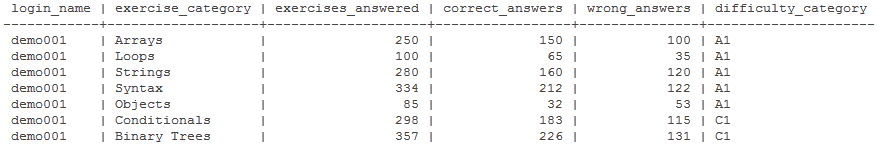
\includegraphics[width=\textwidth,height=\textheight,keepaspectratio]{performance_database_table}
\caption{Performance database table.}
\label{fig:performance_database_table}
\end{figure}

Figure \ref{fig:performance_database_table} shows that, for every student, the system records the number of exercises answered, the number of correct answers and the number of wrong answers for each exercise category defined by the teacher. In addition, the system keeps track of what difficulty category the student has reached for every exercise category. This is the information that gets displayed in the pie charts and performance table.

\begin{figure}[H]
\centering
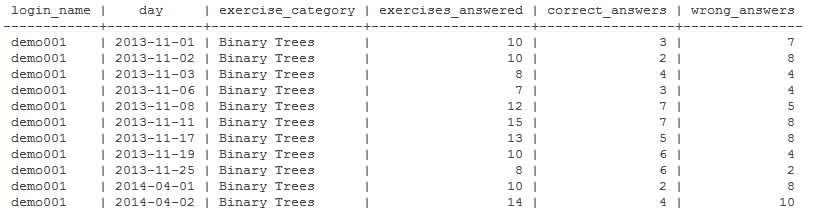
\includegraphics[width=\textwidth,height=\textheight,keepaspectratio]{history_database_table}
\caption{History database table.}
\label{fig:history_database_table}
\end{figure}

Figure \ref{fig:history_database_table} shows that the system records, for every student, the days where exercises were answered, the number of exercises answered answered on that day, the number of correct answers and the number of wrong answers, for every exercise category. This data is used to plot the stacked bar charts of monthly and yearly progress.

\begin{figure}[H]
\centering
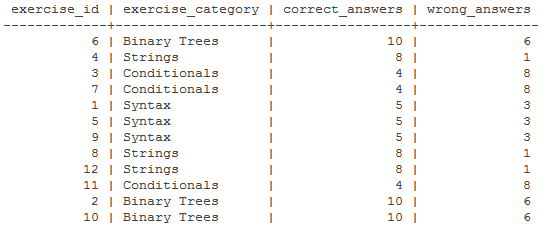
\includegraphics[width=\textwidth,height=\textheight,keepaspectratio]{exercisebank_database_table}
\caption{Exercise bank database table.}
\label{fig:exercisebank_database_table}
\end{figure}

Figure \ref{fig:exercisebank_database_table} shows that the system records the number of correct answers and wrong answers for each exercise. This is a useful feature for teachers to identify trends in which type of exercises students are having trouble with and which type of exercises students are having little trouble answering correctly.

\section{Summary}

\newpage

Talk about design choices such as only multiple choices, no exercises asking to write code, writing custom server, etc...\newline

java programming exercises, binary trees and code exercises to show the capabilities of the system, that it can handle multiple types of exercises.\newline

showing feedback immediately after the exercise....cite source, shown to be most effective way of learning\newline

piece of code + exercise involving the behaviour of the code have been found efficient (lister 2001) as far as student's assessment on their ability to read and understand the code's semantics. (NOT MY OWN WORDS) Lister, R. (2001). Objectives and objective assessment in CS1. ACM SIGCSE Bulletin, Vol. 33, No. 1, pp. 292-296. \newline

CAT development, we refer back to the five components of a CAT...what item selection algorithm we use, what scoring procedure, no termination criterion, entry point is average knowledge distribution initially and attempts at a calibrated item pool, currently with teacher providing the parameters since obtaining a high quality calibrated item pool isn't something I can do.


%-----------------------------------------------------------
% EVALUATION SECTION
%-----------------------------------------------------------
\chapter{Evaluation}
\label{chap:evaluation}
In this chapter we evaluate the strengths and weaknesses of jSCAPE and its various components and features, with respect to the objectives we set at the beginning of the project.

\section{Evaluating jSCAPE}
\subsubsection{Evaluating the graphical user interface}
When justifying our choices for technologies, we mentioned that one of the reasons for using Java applets and JavaFX was to provide a user-friendly and visually appealing user interface. Evidence\cite{Interface-study} suggests that students will prioritise a visually appealing user interface over powerful features. Therefore, we must make sure that our interface is generally well received amongst students, for jSCAPE to be actually useful.\newline

A small amount of data was gathered during an undergraduate fair on 02/06/2014, and during a meeting with student friends on 07/06/2014. In total we asked 10 students what they thought of the jSCAPE interface. The comments were mostly positive, however a few students mentioned that the interface was too large, requiring full screen at times. Two students also mentioned that we should be careful not to overload the view with information, particularly the Profile tab where all the statistics are displayed. We would need more data to identify possible improvements, if any, in the user interface. \newline

We didn't ask for feedback on the user interface of the admin tool as we feel this is less of a factor when it comes to whether teachers actually use the tool. Nonetheless, we think that the GUI of the admin tool is sufficiently user friendly for its purpose.

\subsubsection{Evaluating current jSCAPE exercises}
At the time of writing this report, we have implemented four exercise generators for the exercise categories of Binary Trees, Conditionals, Syntax and Strings. Some example exercises are shown in appendix \ref{chap:example-jscape-exercises}. \newline

For Binary Tree exercises, we supply a binary tree as exercise data, and ask the student to select what is printed after a specific traversal order. This type of exercise was intended to show that it was possible to bring variety to jSCAPE exercises. We think that this exercise is useful for learning the different traversal orders, however the exercise loses its usefulness very quickly once a student has mastered traversal orders. Perhaps this exercise would be more effective if we asked the student to type in the whole traversal instead of selecting the correct answer among the four different traversals.\newline

Next, for Conditionals and Strings exercises, we display a code snippet as exercise data, and ask the student to determine the final value of one or more variables. The usefulness of this type of exercise has been demonstrated in research. Indeed, \cite{Lister} has shown that this type of exercise provides effective assessment on a student's understanding of code semantics.\newline

Thanks to our random code generators, jSCAPE is able to provide many of such exercises, with very different code snippets. This means that a teacher could automatically generate 1000 Conditionals exercises and all of them would include very different code snippets, thus providing students with a large supply of exercises to self-assess their understanding of control flow in Java. However, sometimes the generated code can end up being too random, and the control flow doesn't resemble anything that would appear in a ``real" program. As such, more work would be needed in the code generating component, to make the generated code more useful in the learning process. \newline

Finally, Syntax exercises also present a code snippet, but this time containing syntax errors. The exercise asks the student to spot the syntax error, or to identify how many syntax errors the piece of code contains. We believe that this is a useful exercise for students to familiarise themselves with the Java language, especially in the early stages, when students are discovering programming languages for the first time. \newline

We would like to point out that teachers and educators have more knowledge of what constitutes a useful exercise in assessing students knowledge of a particular concept. These exercises were only intended to show what can be achieved in the jSCAPE system.

\subsubsection{Evaluating the jSCAPE exercise format}
The jSCAPE exercise format was sufficient for us to implement four exercise generators for multiple choice type questions. The format is quite flexible to allow for different views to be used in providing exercise data to accompany the question. The format was also designed with other exercise types in mind. For instance, if the exercise displayer were to read \textsf{FillInBlank} in the \textsf{$<$view$>$} tag of the second \textsf{$<$display$>$} tag, then it would ignore all the \textsf{$<$choice$>$} tags and simply create a text field for the student to type in his answer. \newline

However, in general we are not that satisfied with the exercise format. It isn't very elegant and we could see it posing some restrictions in the future. \newline

\begin{lstlisting}[language=xml, caption={A modified exercise format.}, label=lst:new_exercise_format]
<?xml version="1.0"?>
<exercise>
	<display>
		<view>........</view>
		<value>.......</value>
	</display>
	<display>
		<view>........</view>
		<value>.......</value>
	</display>
	<display>
		<view>........</view>
		<value>.......</value>
	</display>
</exercise>
\end{lstlisting}

We believe that it should be modified to allow for more exercise types to be added to jSCAPE. The listing in \ref{lst:new_exercise_format} shows a possible modification, which makes the exercise format more straightforward. Each possible \textsf{$<$view$>$} could have a component implemented in Java which takes as parameter the value of the \textsf{$<$value$>$} tag. This is how the \textsf{BinaryTree} and \textsf{CodeEditor} were implemented, but for some unknown reason, we didn't think about doing the same with other views such as \textsf{MultipleChoice}. This would offer a more general purpose exercise format than jSCAPE currently has at the moment.\newline

In addition, we designed exercises as consisting of exercise data in the left window, and the question and choices in the right window. This format is also a bit restrictive as it doesn't allow more interactive types of exercises which would require drag and drop functionality, for instance.

\subsubsection{Evaluating automated exercise generation}
Exercises of the Binary Trees category were very suitable for automated generation. Indeed, generating random binary trees with a random number of nodes is something relatively easy to do, and the randomness of the binary tree doesn't impact the quality of the exercise.\newline

For exercises which display code snippets, we mentioned before that this generated code can sometimes be too random, and that ``strange" code can sometimes be produced. This can definitely impact the quality and effectiveness of the exercise. For instance, sometimes an \textsf{if} branch would contain the statement \textsf{var6=true} followed by the exact same statement on the next line. This kind of statement would never appear in a program written by a competent programmer, thus presenting this code snippet to a student could very well be counter productive. \newline

We believe that we have shown how exercise generators can be written to provide, theoretically, endless amounts of exercises. This was one of the objectives we set for the project at the beginning of development. However, it still remains that an exercise generator must be written manually for each new type of exercise. This isn't a very scalable solution, and thus we discuss some possible improvements for automated exercise generation, in the next chapter.

\subsubsection{Evaluating computerized adaptive testing in jSCAPE}
As part of adapting the difficulty of exercises to the student's ability, we implemented two exercise selection algorithms, one based on difficulty categories and another one based on Item response theory.\newline

The difficulty category idea was inspired by PAT\cite{PAT} and we improved the algorithm to include it in jSCAPE. The improvement was based on evidence\cite{Abdullah} which suggests that at most three exercises of a given difficulty are needed to remove uncertainty from assessing a student's knowledge.\newline

The algorithm performed well, thanks to the state machine implementation it is correct in that it will always choose an exercise of the appropriate difficulty category. It is less sophisticated than the Item response theory based algorithm, however it is much easier for teachers, because all they have to do is assign the exercise to one of three categories. But the fact that there are only three exercise categories means that there is less distinction between the difficulty of exercises, as opposed to IRT where we had 11 difficulty levels and the discrimination parameter which also affected perceived difficulty.\newline

Difficulty categories could also be assigned through the automated exercise generation process. To do this we used simple metrics such as binary tree size, code length or number of variables. This worked well under the assumption that Binary Tree exercises become more difficult as they grow in size or as they become unbalanced, however we aren't sure this assumption is valid. It may be valid early on when students are learning about binary trees for the first time. \newline

Exercises with code snippets were much more suitable for automatically assigning to a difficulty category because more metrics were available. For Conditionals, we used the number of \textsf{if/else} branches and the number of variables asked for. This worked quite well, however the randomness of the code would still interfere sometimes. A more sophisticated code analysis would be needed to determine the difficulty category and we discuss some improvements in the next chapter.\newline

The more sophisticated exercise selection algorithm we implemented was based on Item response theory. We managed to test the correctness of the implemented algorithm by running a simulation, whose results are included in appendix \ref{chap:irt-simulation}. It shows that the algorithm does indeed choose the most appropriate exercise according to the student's estimated knowledge level. The knowledge distribution is also updated correctly.\newline

However, this solution did present some limitations, most notably, it requires teachers to input the item parameters, that is the difficulty and discrimination parameters. Although guidelines were given for this step, the results will be a lot less accurate than what could be achieved through using calibration software and data. Still, it provides a bit more options than the difficulty category based method. \newline

We also evaluate our system in terms of the advantages and disadvantages mentioned in CAT (section \ref{sec:CAT}). Most of the complaints for CATs are for when they are used as means to assess students for a grade which counts towards their end of year total. For instance, not being able to go back and change one's answer. In a self-assessment setting, where the results don't really count towards anything, this isn't much of a problem. However, jSCAPE does present the most common weakness of CATs, in that a large bank of calibrated exercises is needed to be effective. Finally, we mentioned that exercise exposure could be an issue in CATs, but in jSCAPE we aren't concerned about this, because the system is only intended for self-assessment.

\subsubsection{Evaluating collection of statistical data}
To determine which statistics should be collected by jSCAPE, we inspired ourselves from other software, in particular video games, with statistics such as win/losses, history over time, etc...In addition, we regularly received feedback from our supervisor, Dr. Tristan Allwood, in terms of which statistics would be useful for a teacher or lecturer in monitoring students' progress. Asking more lecturers or teachers could help in determining more useful statistics that jSCAPE could record and display to students or teachers. It would be quite easy to add more statistics, however we believe that the core useful statistics have been implemented.

\section{Summary}
In this chapter we evaluated the different components that form the jSCAPE system. We showed that collection and display of statistical data was implemented quite solidly, and that the system was able to support provision of exercises very well.\newline

However, jSCAPE did present certain limitations in its exercise format, in its exercise generators and in the adaptive difficulty component. \newline

In the next chapter we conclude the project and give some possibilities of future work which could address the weaknesses of the system discussed in this section.

%-----------------------------------------------------------
% CONCLUSION SECTION
%-----------------------------------------------------------
\chapter{Conclusion}
\section{Future Work}
We have a few ideas of where to orient the project next...

\begin{itemize}
\item Very flexible system so other programming languages could be offered, i.e. cSCAPE, for C and hSCAPE for Haskell. 
\item Working more extensively on the adaptive component of the system, i.e. improving the algorithm which selects questions for students based on their estimated ability.
\item Extend system to allow admins to provide their own question templates, maybe come up with a template grammar which then allows questions to be automatically generated. Or at least allow pluggable function references which will be called to generate the exercise component.
\item Add support for more question types. JavaFX is very good in that sense since it can play audio clips, video clips, show animations, the webview component has endless possibilities thanks to the inclusion of Javascript.
\item Future Work as a research project vs future work as a commercial product
\item JavaFX applications are based on the model-view-controller pattern, so a nice split can be done in the code, however I only learnt about this two weeks into the project, so all the of the GUI components are created in the code as opposed to in the FXML file.
\item add more robust security: hashing for login/password and ssl connections between the server and client, and server database, because this communication could reveal solutions to the exercises..
\end{itemize}

%-----------------------------------------------------------
% Bibliography
%-----------------------------------------------------------
\begin{thebibliography}{9}

\bibitem{SIETTE} Conejo, R., Guzmán, E., Millán, E., Trella, M., Pérez-de-la-Cruz, J. L., \& Rios, A. (2004). SIETTE: A Web-Based Tool for Adaptive Testing. \textit{International Journal of Artificial Intelligence in Education, 14}, 29-61.

\bibitem{CAT-Wiki} Computerized adaptive testing. \url{http://en.wikipedia.org/wiki/Computerized_adaptive_testing}. Accessed: \today.

\bibitem{CAT-Framework} Thompson, Nathan A., \& Weiss, David A. (2011). A Framework for the Development of Computerized Adaptive Tests. \textit{Practical Assessment, Research \& Evaluation}, 16(1).

\bibitem{CAT-Areas} IRT-Based CAT. \url{http://www.iacat.org/content/irt-based-cat}. Accessed: \today.

\bibitem{Weiss1984} Weiss, D. J., \& Kingsbury, G. G. (1984). Application of computerized adaptive testing to educational problems. \textit{Journal of Educational Measurement}, 21, 361-375

\bibitem{Weiss1985} Weiss, D.J. (1985). Adaptive Testing by Computer, \textit{Journal of Consulting and Clinical Psychology}. 1985, 53, 6, pp. 774-789.

\bibitem{CAT-Primer} Wainer, H., \& Mislevy, R.J. (2000). Item response theory, calibration, and estimation. In Wainer, H. (Ed.) Computerized Adaptive Testing: A Primer. Mahwah, NJ: Lawrence Erlbaum Associates.

\bibitem{IRT-Wiki} Item Response Theory. \url{http://en.wikipedia.org/wiki/Item_response_theory}. Accessed: \today.

\bibitem{Basics-IRT} Baker, Frank (2001). The Basics of Item Response Theory. (2nd Edition). Available at \url{http://info.worldbank.org/etools/docs/library/117765/Item\%20Response\%20Theory\%20-\%20F\%20Baker.pdf}. Accessed: \today.

\bibitem{Visual-IRT} Partchev, Ivailo (2004). A visual guide to item response theory. Available at \url{www.metheval.uni-jena.de/irt/VisualIRT.pdf}. Accessed: \today.

\bibitem{PAT} Chatzopoulou, D. I. \& Economides, A. A. (2010). Adaptive assessment of student's knowledge in programming courses. \textit{Journal of Computer Assisted Learning}, Vol. 26, No. 4.

\bibitem{SIETTE-small} Guzman, E.; Conejo, R., Self-assessment in a feasible, adaptive web-based testing system, Education, \textit{IEEE Transactions}, vol.48, no.4, pp.688,695, Nov. 2005.

\bibitem{SIETTE-components} E. Guzmán and R. Conejo, A brief introduction to the new architecture of SIETTE, in \textit{Lecture Notes in Computer Science. Proc. 3rd Adaptive Hypermedia Adaptive Web-based Systems (AH 2004)}, Berlin, Germany,
2004.

\bibitem{Interface-study} Christine Phillips \& Barbara S. Chaparro. Visual Appeal vs. Usability: Which One Influences User Perceptions of a Website More? \url{http://psychology.wichita.edu/surl/usabilitynews/112/aesthetic.asp}. Accessed: \today.

\bibitem{JavaFX} JavaFX - The Rich Client Platform. \url{http://www.oracle.com/technetwork/java/javase/overview/javafx-overview-2158620.html}. Accessed: \today.

\end{thebibliography}

%-----------------------------------------------------------
% APPENDICES
%-----------------------------------------------------------
\appendix
\chapter{Example jSCAPE exercises}
\label{chap:example-jscape-exercises}

\subsubsection{Binary tree exercise}
\lstinputlisting[language={xml}, tabsize=4, caption={Example exercise for the Binary Tree exercise category}]{\listings/binary_tree_exercise.xml}

\subsubsection{Strings exercise}
\lstinputlisting[language={xml}, tabsize=4, caption={Example exercise for the Strings exercise category.}]{\listings/strings_exercise.xml}

\subsubsection{Conditionals exercise}
\lstinputlisting[language={xml}, tabsize=4, caption={Example exercise for the Conditionals exercise category}]{\listings/conditionals_exercise.xml}

\chapter{Item Response Theory Simulation}
\label{chap:irt-simulation}
\begin{verbatim}
run:
Item 1, a=0.600000024, b=2.0, c=0.25
Item 2, a=1.10000002, b=5.0, c=0.25
Item 6, a=1.20000005, b=6.0, c=0.25
Item 4, a=1.39999998, b=10.0, c=0.25
Item 7, a=1.29999995, b=8.0, c=0.25
Item 8, a=1.29999995, b=9.0, c=0.25
Item 9, a=1.29999995, b=8.0, c=0.25
Item 10, a=1.20000005, b=7.0, c=0.25
Item 3, a=0.899999976, b=4.0, c=0.25
Item 5, a=1.10000002, b=6.0, c=0.25
Item 11, a=0.899999976, b=5.0, c=0.25
Item 13, a=1.20000005, b=6.0, c=0.25
Item 12, a=1.20000005, b=7.0, c=0.25
Item 14, a=1.20000005, b=5.0, c=0.25
Item 19, a=1.10000002, b=8.0, c=0.25
Item 16, a=0.899999976, b=4.0, c=0.25
Item 20, a=1.10000002, b=6.0, c=0.25
Item 17, a=1.0, b=6.0, c=0.25
Item 18, a=1.0, b=6.0, c=0.25
Item 15, a=1.10000002, b=8.0, c=0.25

Initial ability estimate is 5.0
Response pattern: 1,1,0,1,1,0,1,0,0,1,1,1,1

ItemID with max information=14....item difficulty = 5.0
Answering item correctly...
Level 0; p(X) = 0.03636769115505164
Level 1; p(X) = 0.037206623471527936
Level 2; p(X) = 0.038260317342103396
Level 3; p(X) = 0.04081036191593649
Level 4; p(X) = 0.05349299152794003
Level 5; p(X) = 0.10165259009990486
Level 6; p(X) = 0.1468438899647491
Level 7; p(X) = 0.1455581552386823
Level 8; p(X) = 0.13531360399937065
Level 9; p(X) = 0.12710657491229954
Level 10; p(X) = 0.12100612155365803
After answering item, theta estimate is now 6

ItemID with max information=6....item difficulty = 6.0
Answering item correctly...
Level 0; p(X) = 0.013124740793219158
Level 1; p(X) = 0.013542401445264645
Level 2; p(X) = 0.014057388340824017
Level 3; p(X) = 0.015215361137360064
Level 4; p(X) = 0.02100213737667263
Level 5; p(X) = 0.051797448304890685
Level 6; p(X) = 0.14268364973784606
Level 7; p(X) = 0.20760489960552594
Level 8; p(X) = 0.1916296772375679
Level 9; p(X) = 0.16853841728581867
Level 10; p(X) = 0.15231185483440784
After answering item, theta estimate is now 7

ItemID with max information=10....item difficulty = 7.0
Answering item incorrectly...
Level 0; p(X) = 0.03426092158943807
Level 1; p(X) = 0.03350256540359772
Level 2; p(X) = 0.03313907735209839
Level 3; p(X) = 0.03431631472252459
Level 4; p(X) = 0.04532468027557683
Level 5; p(X) = 0.10467277882139388
Level 6; p(X) = 0.23442418103313054
Level 7; p(X) = 0.16747623219413782
Level 8; p(X) = 0.03676628018469355
Level 9; p(X) = 0.004815402028441693
Level 10; p(X) = 5.768602180674826E-4
After answering item, theta estimate is now 6

ItemID with max information=13....item difficulty = 6.0
Answering item correctly...
Level 0; p(X) = 0.02028756239063162
Level 1; p(X) = 0.020005962646609306
Level 2; p(X) = 0.019964567998580075
Level 3; p(X) = 0.02095836406139418
Level 4; p(X) = 0.029109831216476114
Level 5; p(X) = 0.08704278780210205
Level 6; p(X) = 0.3676788788796302
Level 7; p(X) = 0.31762619226094463
Level 8; p(X) = 0.058659118650767436
Level 9; p(X) = 0.007504854463641741
Level 10; p(X) = 8.965732158816038E-4
After answering item, theta estimate is now 6

ItemID with max information=5....item difficulty = 6.0
Answering item correctly...
Level 0; p(X) = 0.007921854133211843
Level 1; p(X) = 0.007851530701417237
Level 2; p(X) = 0.007884102039918992
Level 3; p(X) = 0.008393036691102489
Level 4; p(X) = 0.012396255823329205
Level 5; p(X) = 0.048885794487403086
Level 6; p(X) = 0.376655920288866
Level 7; p(X) = 0.4641986540411844
Level 8; p(X) = 0.0770970854357723
Level 9; p(X) = 0.009774176795030516
Level 10; p(X) = 0.0011669386976239583
After answering item, theta estimate is now 7

ItemID with max information=12....item difficulty = 7.0
Answering item incorrectly...
Level 0; p(X) = 0.011877887469279843
Level 1; p(X) = 0.011702978802794266
Level 2; p(X) = 0.011684072562684555
Level 3; p(X) = 0.012365574101473823
Level 4; p(X) = 0.018122648551965423
Level 5; p(X) = 0.06984984926009075
Level 6; p(X) = 0.47022057826311203
Level 7; p(X) = 0.29318522593170404
Level 8; p(X) = 0.012563089704461445
Level 9; p(X) = 2.3258255458602479E-4
Level 10; p(X) = 3.6644645983882904E-6
After answering item, theta estimate is now 6

ItemID with max information=20....item difficulty = 6.0
Answering item correctly...
Level 0; p(X) = 0.004855919229956476
Level 1; p(X) = 0.0047992460547199075
Level 2; p(X) = 0.004811970748426527
Level 3; p(X) = 0.0051542622134070825
Level 4; p(X) = 0.008016402606395278
Level 5; p(X) = 0.040641160894608244
Level 6; p(X) = 0.49678042634666586
Level 7; p(X) = 0.43378398292523146
Level 8; p(X) = 0.016802005427202126
Level 9; p(X) = 3.139215345169494E-4
Level 10; p(X) = 4.956930909540798E-6
After answering item, theta estimate is now 6

ItemID with max information=17....item difficulty = 6.0
Answering item incorrectly...
Level 0; p(X) = 0.012857979860137338
Level 1; p(X) = 0.012442169512784512
Level 2; p(X) = 0.0122216494348138
Level 3; p(X) = 0.012785562238543855
Level 4; p(X) = 0.019000760832745923
Level 5; p(X) = 0.08203210562478577
Level 6; p(X) = 0.547234697520948
Level 7; p(X) = 0.13984693166143292
Level 8; p(X) = 0.0012510896478464977
Level 9; p(X) = 4.391050717578476E-6
Level 10; p(X) = 1.2729688571107645E-8
After answering item, theta estimate is now 6

ItemID with max information=18....item difficulty = 6.0
Answering item incorrectly...
Level 0; p(X) = 0.029678874782892165
Level 1; p(X) = 0.027641126423564
Level 2; p(X) = 0.02624051311476951
Level 3; p(X) = 0.026517157227254406
Level 4; p(X) = 0.037304834991676875
Level 5; p(X) = 0.135841766493143
Level 6; p(X) = 0.49202963517146353
Level 7; p(X) = 0.04087346140850065
Level 8; p(X) = 7.872920151215608E-5
Level 9; p(X) = 5.1851911423047384E-8
Level 10; p(X) = 2.7597504092165085E-11
After answering item, theta estimate is now 6

ItemID with max information=2....item difficulty = 5.0
Answering item correctly...
Level 0; p(X) = 0.01218621570180688
Level 1; p(X) = 0.011447973091770907
Level 2; p(X) = 0.011042318093585394
Level 3; p(X) = 0.011882275557934254
Level 4; p(X) = 0.02203393938987174
Level 5; p(X) = 0.1445151599655469
Level 6; p(X) = 0.7467401069214272
Level 7; p(X) = 0.04885256915234908
Level 8; p(X) = 9.460065717340942E-5
Level 9; p(X) = 6.244833073308885E-8
Level 10; p(X) = 3.324920495966649E-11
After answering item, theta estimate is now 6

ItemID with max information=11....item difficulty = 5.0
Answering item correctly...
Level 0; p(X) = 0.003788639987107719
Level 1; p(X) = 0.0035868035884545025
Level 2; p(X) = 0.0035494662597438304
Level 3; p(X) = 0.004215996938004986
Level 4; p(X) = 0.010600922414678006
Level 5; p(X) = 0.11394109994797201
Level 6; p(X) = 0.8364204181699381
Level 7; p(X) = 0.05545773866937719
Level 8; p(X) = 1.0946553006657731E-4
Level 9; p(X) = 7.268882619609612E-8
Level 10; p(X) = 3.875146904084948E-11
After answering item, theta estimate is now 6

ItemID with max information=3....item difficulty = 4.0
Answering item correctly...
Level 0; p(X) = 9.795168022923113E-4
Level 1; p(X) = 9.497394751603832E-4
Level 2; p(X) = 0.0010356521315317583
Level 3; p(X) = 0.001664706600190618
Level 4; p(X) = 0.006828712076886231
Level 5; p(X) = 0.10200537508217888
Level 6; p(X) = 0.844156542398744
Level 7; p(X) = 0.057034236666960246
Level 8; p(X) = 1.1306244281980126E-4
Level 9; p(X) = 7.517390516847282E-8
Level 10; p(X) = 4.008750839724127E-11
After answering item, theta estimate is now 6

ItemID with max information=16....item difficulty = 4.0
Answering item correctly...
Level 0; p(X) = 2.5500873149534046E-4
Level 1; p(X) = 2.5309431275512853E-4
Level 2; p(X) = 3.039646180160208E-4
Level 3; p(X) = 6.608577852321254E-4
Level 4; p(X) = 0.004419795981432214
Level 5; p(X) = 0.0916758728146013
Level 6; p(X) = 0.8540744186749987
Level 7; p(X) = 0.05867119922756449
Level 8; p(X) = 1.1680139881184215E-4
Level 9; p(X) = 7.775981216800935E-8
Level 10; p(X) = 4.1478074941804744E-11
After answering item, theta estimate is now 6

BUILD SUCCESSFUL (total time: 1 second)
\end{verbatim}

\chapter{IRTModule.java}
\label{chap:irt-module}
\lstinputlisting[language=Java, caption={Item Response Theory module.}]{\listings/irt_module.java}

\end{document}